\section{Uncertainty budget}\label{ch:Uncertainty}

\section{Outline Of the Measurement}
If LArIAT had a beam of pure pions and were 100\% efficient in determining the interaction point within the TPC, the pion cross section in each energy bin would be given by

\begin{equation}
 \sigma_{TOT}(E_{i})  = \frac{1}{n \delta X}\frac{N_{Interacting} (E_{i})}{N_{Incident}(E_{i})}.
\label{eq:thinTargetXSSolved}
\end{equation}

Unfortunately, this is not the case. The selection used to isolate pions in the LArIAT beam allows for the presence of some muons and electrons as contaminants. Also, the LArIAT TPC is not 100\% efficient in determining the interaction point. Therefore we need to apply two corrections in order to extract the true pion cross section from LArIAT data: the background subtraction and the efficiency correction. 
We estimate the true pion cross section in each energy bin would changing  the equation \ref{eq:thinTargetXSSolved} into
\begin{equation}
 \sigma^{\pi^-}_{TOT}(E_{i})  = \frac{1}{n \delta X}\frac{ \epsilon^{inc}_i [ N_{Interacting} (E_{i}) - B_{interacting} (E_i)] }{   \epsilon^{int}_i [N_{Incident}(E_{i}) - B_{incident} (E_i)]},
\label{eq:True}
\end{equation}

where $B_{interacting} (E_i)$ and $B_{incident} (E_i)$ represent the contributions from beamline contaminants to the interacting and incident histograms respectively, and  $\epsilon^{int}_i$ and  $\epsilon^{inc}_i$ are the efficiency corrections for said histograms.

The following sections describe the procedures used to evaluate  the background subtraction \ref{sec:beamCont} and the efficiency correction \ref{sec:EffCorrection}  and the estimate of their uncertainties. 
The reader might be concerned about bin-by-bin migration of events in the interacting and incident plots due to the finite resolution of the energy reconstruction. In \ref{sec:Energy}, we make an argument to why we expect the smearing matrix to be extremely close to diagonal and its calculation is left for an improvement of the current analysis.



\section{Handling Beamline Contamination}\label{sec:beamCont}




\section{Tracking Studies}
\subsection{Angular Resolution}
Scope of this study is to understand and compare the tracking performances and angular resolution of the TPC tracking on data and MC. 
We use the angular resolution of the tracking to determine  the value of smallest angle that we can reconstruct with a non-zero efficiency, effectively determining a selection on the angular distribution of the cross section measurement due to the tracking performances.


We use the same procedure to evaluate the tracking performance in data and MC  outlined in this section. 
We start by selecting all the WC2TPC matched tracks, that are the tracks used for the cross section analysis.  These tracks can contain from a minimum of 3 3D-space points to a maximum of 240  3D-space points.  We fit a line to all the 3D space points associated with the track. 
For each track we calculate the average distance between each 3D point in space and the fit line as follows 
\begin{equation} 
\bar d = \frac{\sum^N_i d_i}{N},
\end{equation} 
where $N$ is the number of point of the track and $d_i$ is the distance of the $i$-th space point to the line fit. Several tests to compare the goodness of fit between data and MC have been considered. We decided to use $\bar d$ for its straightforward interpretation. The $\bar d$ distribution for data and MC is shown in Figure \ref{fig:Chi2AllPts}.

A visual representation of the procedure used to evaluate the angular resolution is shown in Figure \ref{fig:AngResProcedure}. 
For each track, we order the space points according to their Z position (along the positive beam direction) and we split them in two sets: the first set contains all the points belonging to the first half of the track and the second set counts all the points contains to the second half of the track. We remove the last four points in the first set and the first four points in the second set, so to have a gap in the middle of the original track. We fit the first and the second set of points with a line separately. We then calculate the angle between the fit of the first and second half $\alpha$. The angle $\alpha$ determines the spatial resolution of the tracking. The distributions for data and MC for $\alpha$ are given in \ref{fig:trackingResolution}. The mean of the data and MC angular resolution are respectively 

\begin{equation}
\bar\alpha_{Data} = (4.7 \pm 3.3) \text{ deg} 
\end{equation}

\begin{equation}
\bar\alpha_{MC} = (4.5 \pm 3.2) \text{ deg}. 
\end{equation}

A small, $0.2 \text{ deg}$ systematic shift between the mean of the data and MC angular resolution is present, which we account for in the context of the MC efficiency correction to the cross section, as presented in \ref{sec:angSys}.


\begin{figure}[htb]
\centering
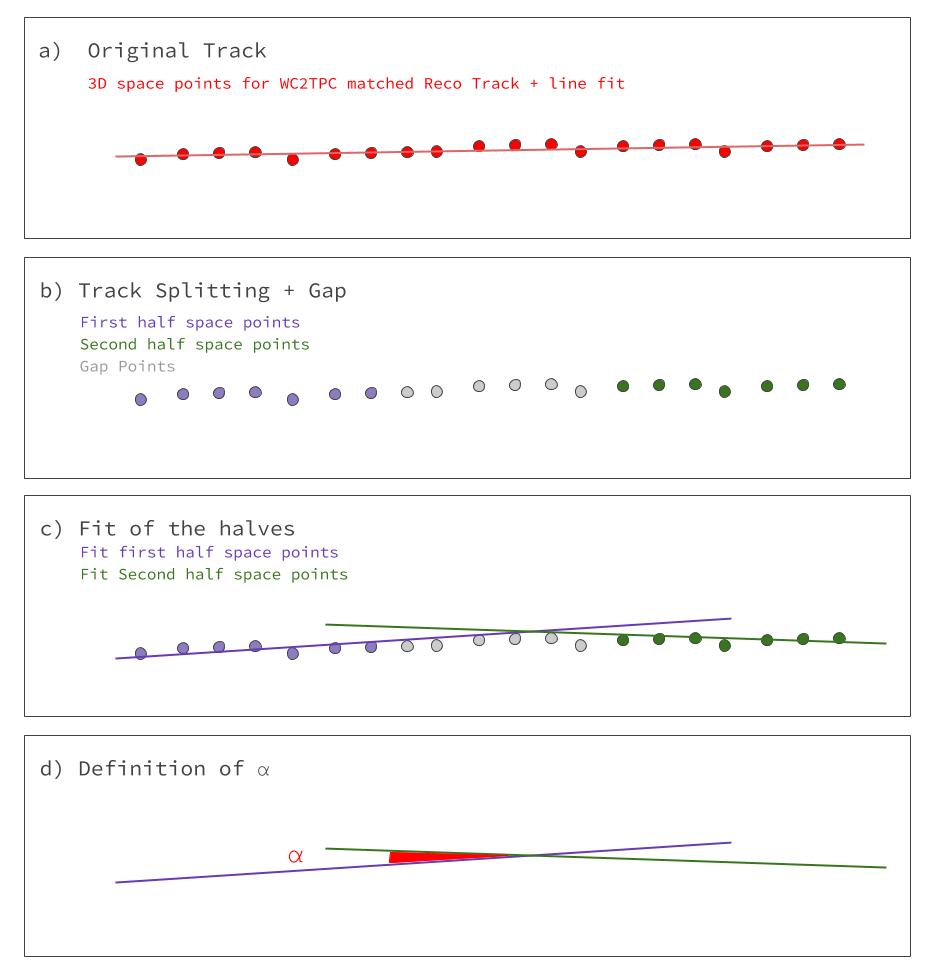
\includegraphics[width=\textwidth]{Studies/Figures/TrackingProcedure.png}
\caption[]{ Sketch of the procedure used to determine the angular resolution. } \label{fig:AngResProcedure}
\end{figure}


\begin{figure}[htb]
\centering
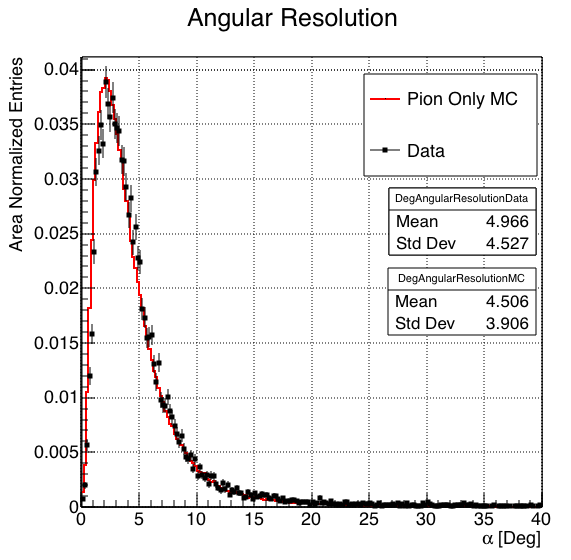
\includegraphics[width=0.48\textwidth]{Studies/Figures/cTrackingDeg.png}
\caption[]{Distributions of angular resolution $\alpha$ for data used in the pion cross section analysis and pion only DDMC. The distributions are area normalized. } \label{fig:trackingResolution}
\end{figure}


\section{Efficiency Correction}\label{sec:EffCorrection}.

\subsection{Systematics on Efficiency Correction}\label{sec:angSys}.


%%%%%%%%%%%%%%%%%%%%%%%%%%%%%%%%%%%%%%%%%%%%%%%%%%%%%%%%
\begin{comment}
Assuming a beam of pure pions gets to the TPC, let us explicit some of the variables in the kinetic energy equation \ref{eq:KEj}  to point out the important quantities in the uncertainty budget,

\begin{align}
 E_{j}^{kin} &=  E_{Beam}^{kin}  - E_{loss} - \sum_{i < j} \frac {dE_i}{dx_i}*dx_i\\
                  &=  \sqrt{p^2_{Beam} - m^2_{Beam}} - m_{Beam} - E_{loss} - \sum_{i < j} \frac {dE_i}{dx_i}*dx_i.
\end{align}

\subsection{Uncertainty on $E_{Beam}^{kin}$}
Let us start by discussing the uncertainty on $E_{Beam}^{kin}$. Since we are assuming a beam of pions, the uncertainty on the value of mass of the pion ($m_{Beam}$) as given by the pdg is irrelevant compared to the momentum uncertainties, thus $\delta E_{Beam}^{kin} = \delta p_{Beam}^{kin}$. 
We estimate the momentum uncertainty as follows.

\textcolor{blue}{  
We estimate the uncertainty on a 4-point track. In case of 3-points track, we add an additional 2\% coming from Greg's study. 
Uncertainty on a 4-point track:
\begin{itemize}
\item[-]  Alignment surveys. 1mm misalignment translates to 3\% in overall
\item[-] Doug study dp/p = ~2\% based on field map (docdb 1710)
\item[-] Minerva test beam paper
\end{itemize}
}

\subsection{Systematics on $E_{loss}$}




\textbf{Systematics}
Discrepancies between the real TPC geometry and the simulated geometry can lead to a systematic in the $E_{loss}$ calculation. In particular, we found a difference in the depth of the un-instrumented argon upstream to the TPC front face, the MC geometry reporting $~\sim 3.3$ cm more un-instrumented argon than the TPC survey. For a pion MIP, this depth corresponds to 7.4 MeV which we account for as a double sided systematic in the determination of the pion kinetic energy.

\subsection{Uncertainty on dE/dx and pitch}
We obtain the uncertainty on dE/dx and track pitch by comparing the dE/dx and pitch distributions in data and MC.
\textcolor{blue}{ Currently, MPV MC = 1.70 and MPV DATA = 1.72 MeV/cm (~3\% higher).
TO DO HERE: calculate Argon density from mid-RTD temperature. Compare this  density with MC Argon density. 
Density change  affects dE/dx (in MeV/cm!). Try changing MC density up to ``real one" and see if dEdX agrees between DATA and MC}


\subsection{Uncertainty on track end, aka efficiency correction}
From the MC, we obtain an efficiency correction on the interacting and incident distributions separately. This is done by comparing the MC reconstructed with the true MC deposition on an event by event basis.
This correction is applied bin by bin on the data interacting and incident distributions.
The better our tracking, the smaller this efficiency correction will be. So, step number one is improving the tracking.
\textcolor{blue}{Need to talk to Bruce about this.}
\textcolor{blue}{ I don't understand the angle cut that Dave Schmitz and Jon Paley were so vocal about.}

Now, the key question remains: does the tracking behave in the same way in data and MC? 
We can compare some key plots between reconstructed data and MC which gives us confidence this is true: the track pitch, the tracks straightness and the goodness of fit in data and MC. \textcolor{blue}{ Does such a variable as ``goodness of fit" exists in the tracking? We should ask Bruce.}
\end{comment}


\section{Energy Studies}

A study we did was to look at the difference between DATA/MC in the dE/dX and energy deposited. We basically found there is very little difference between the two and we try to quantify how much the difference is.

%%%%%%%%%%%%%%%%%%%%%%%%%%%%%%%%%%%%%%%%%%%%%%%
\subsection{dE/dX}
%%%%%%%%%%%%%%%%%%%%%%%%%%%%%%%%%%%%%%%%%%%%%%%
Figure \ref{fig:dEdXLinearScale} shows the output of the fit of the Pion MC and the 60 Amp data. The MC is normalized to the data and both are fit to a Landau function. \footnote{The entries at dE/dX = 0 come from an uninitialized variable and can/should be taken out of these plots}

\begin{figure}[htb]
\centering
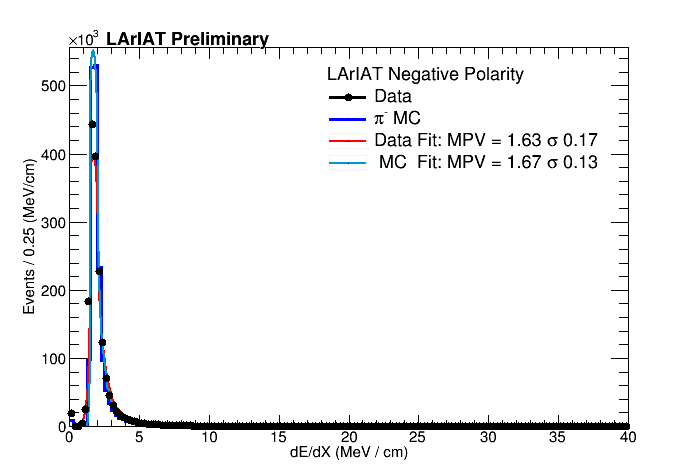
\includegraphics[width=0.48\textwidth]{Studies/Figures/dEdX_Fit_v1.png}
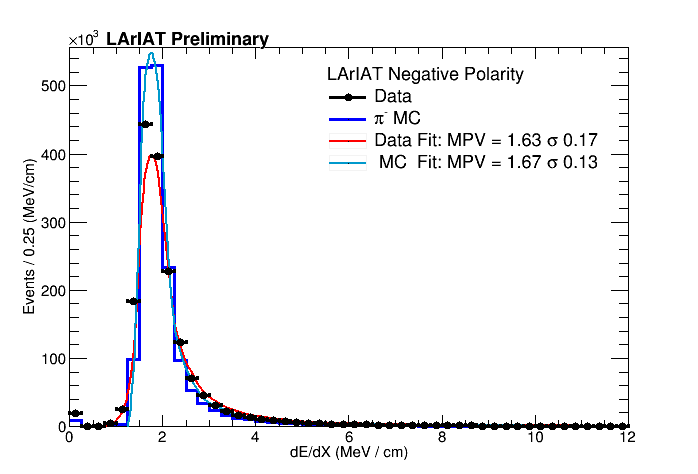
\includegraphics[width=0.48\textwidth]{Studies/Figures/dEdX_Fit_v4.png}
\caption[]{ dE/dX for 60Amp data and data driven pion MC, both fit with a Landau  } \label{fig:dEdXLinearScale}
\end{figure}

The difference between the two MPV's, is 2.4\% between the data and the MC.

Figure \ref{fig:dEdXLinearStacked} shows the stacked version of the dE/dX with the backgrounds stacked. The backgrounds are given in the ratio of 68.8\% pion, 4.6\% muon, and 26.6\% electron. Once they are taken in these ratios, the sum of the MC is normalized to the sum of the data.

\begin{figure}[htb]
\centering
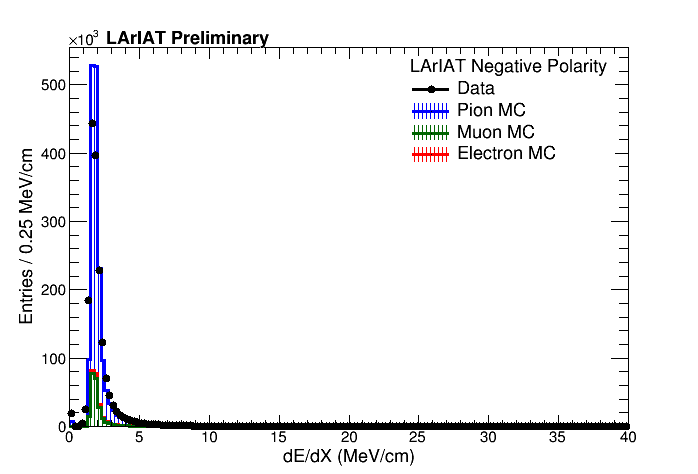
\includegraphics[width=0.48\textwidth]{Studies/Figures/dEdX_stacked_v1.png}
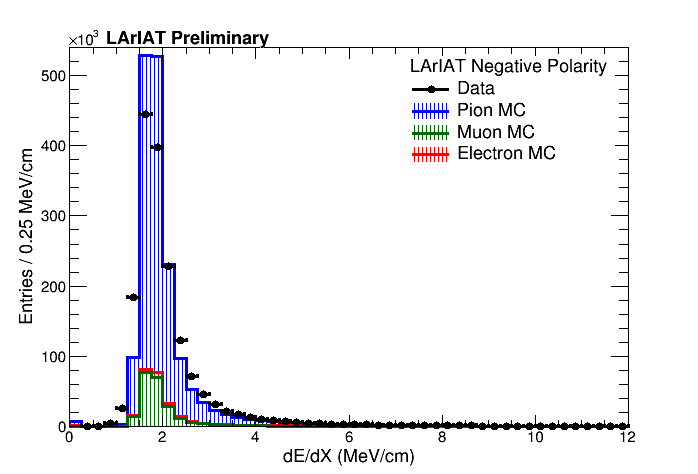
\includegraphics[width=0.48\textwidth]{Studies/Figures/dEdX_stacked_v4.png}
\caption[]{ Stacked versions of the dE/dX with the data and electron/muon/pion MC.  } \label{fig:dEdXLinearStacked}
\end{figure}

For completeness, the log scale versions of are shown in Figure \ref{fig:dEdXLogScale}.

\begin{figure}[htb]
\centering
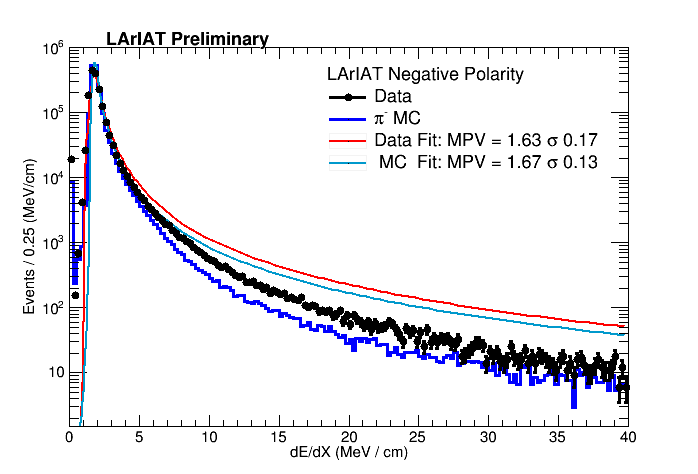
\includegraphics[width=0.48\textwidth]{Studies/Figures/dEdX_Fit_v2.png}
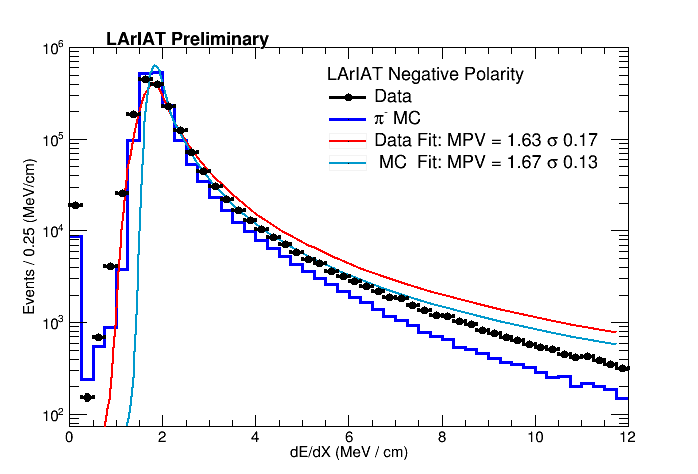
\includegraphics[width=0.48\textwidth]{Studies/Figures/dEdX_Fit_v3.png}
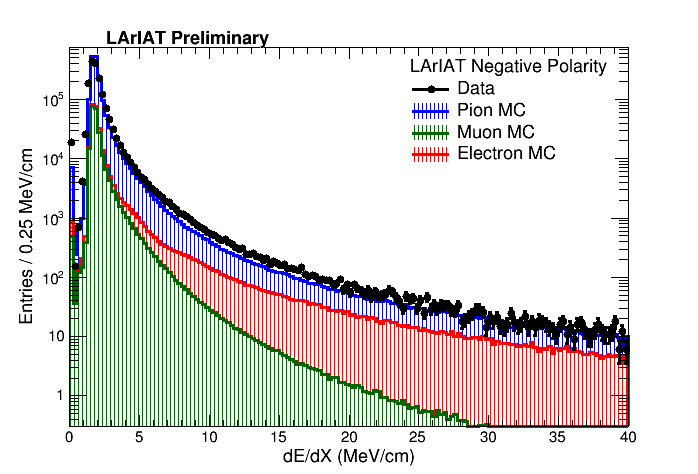
\includegraphics[width=0.48\textwidth]{Studies/Figures/dEdX_stacked_v2.png}
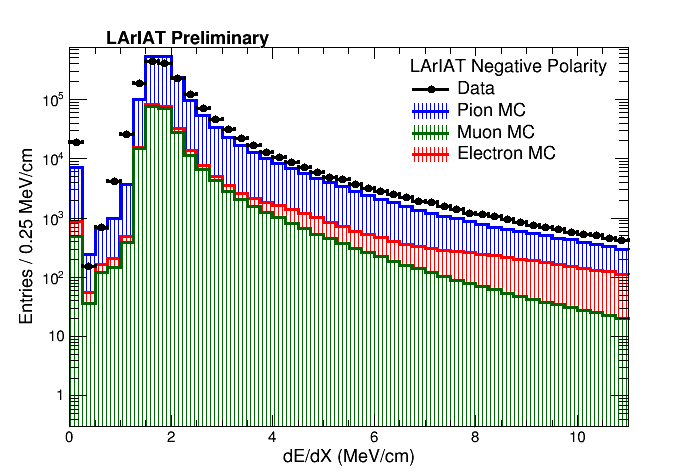
\includegraphics[width=0.48\textwidth]{Studies/Figures/dEdX_stacked_v3.png}
\caption[]{ dE/dX for 60Amp data and MC shown in log scale  } \label{fig:dEdXLogScale}
\end{figure}

Plotting scripts can be found here on lariatgpvm \begin{verbatim}
/lariat/app/users/jasaadi/v06_34_01_PionWeek/PlottingScripts
\end{verbatim} and the samples were put here \begin{verbatim}
/lariat/data/users/elenag/theFinalPions/TPCDATA

/lariat/data/users/elenag/theFinalPions/TPC_MC/
\end{verbatim}

%%%%%%%%%%%%%%%%%%%%%%%%%%%%%%%%%%%%%%%%%%%%%%%
\subsection{Energy Deposited}\label{sec:Energy}
%%%%%%%%%%%%%%%%%%%%%%%%%%%%%%%%%%%%%%%%%%%%%%%
The initial energy the particle has as it enters the TPC is given by

\begin{equation}
KE_{Initial} = \sqrt{P_{WCtrk}^2 + m_{\pi}^2} - m_{\pi}^2 - E_{Loss}
\end{equation}

and the uncertainty of the initial energy $\delta KE_{Initial}$ is given by
\begin{equation}
\delta KE_{Initial} = \sqrt{\delta P_{WCtrk}^2 + \delta E_{Loss}^2}
\end{equation}

If we assume the uncertainty is 2\% as the Minerva experiment had, and our uncertainty on the energy loss upstream is 7~MeV, then the total uncertainty on the initial kinetic energy for a typical 500~MeV pion is $\sim 12$~MeV.

% 17/25 data 24/32 MeV for data with an uncertainty of 7 MeV


Now the energy for $j^{th}$ slab of the incident histogram is given by
\begin{equation}
KE^{Incident}_{j} = KE_{Inital} - (\sum_{i<j} dE/dX_{i} \times Pitch_i)
\end{equation}
where $i$ is given by the slab you are at, $dE/dX_{i}$ is the energy deposited at that slab, and $Pitch_i$ is the pitch for that point. 

Thus we can talk about the energy at the $j^{th}$ slab as 

\begin{equation}
E_{j}^{slab} = (\sum_{i<j} dE/dX_{i} \times Pitch_i)
\end{equation}

The systematic uncertainty of $E_{j}^{slab}$ is given by the difference between this quantity in data and MC, and the uncertainty on $E_{j}^{slab}$ is given by the width of the Landau fit to the data. These are shown in Figure \ref{fig:EnergyDeposited}

\begin{figure}[htb]
\centering
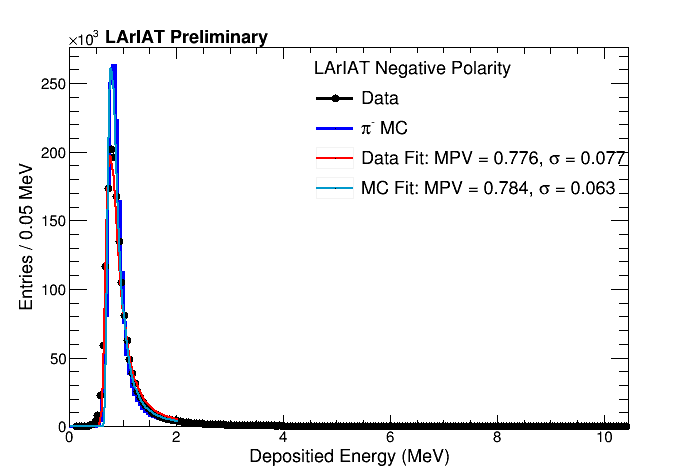
\includegraphics[width=0.48\textwidth]{Studies/Figures/DepEnergy_Fit_v1.png}
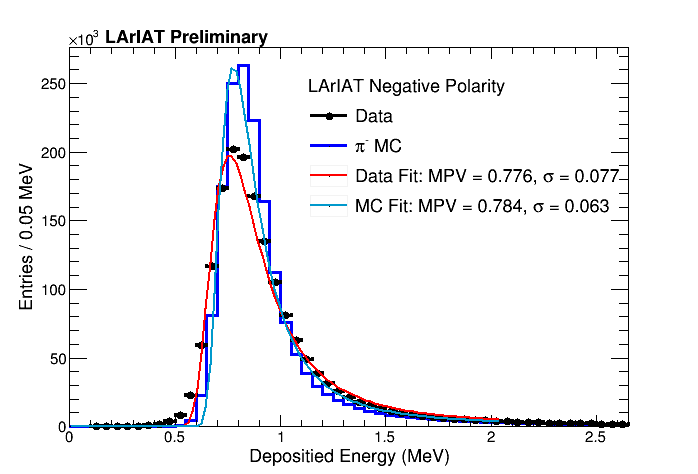
\includegraphics[width=0.48\textwidth]{Studies/Figures/DepEnergy_Fit_v4.png}
\caption[]{ Energy Deposited in Pion MC and 60A data.  } \label{fig:EnergyDeposited}
\end{figure}

The difference between the MPV of data and MC is 1.0\% (0.0784 - 0.0776 / 0.0784) and thus the systematic uncertainty you would assign to the energy in the incident kinetic energy would be for all 240 slices (assuming you have 240 slices at 0.4 mm pitch) and thus is 

\begin{equation}
\delta E^{Slab}_{j} = (0.0784 - 0.0776) \times 240 = 0.008 MeV \times 240 = 1.92 MeV 
\end{equation}

So the uncertainty on the incident kinetic energy is given by

\begin{equation}
\delta KE^{Incident} = \sqrt{ (\delta KE_{Initial})^2 + (\delta E^{Slab}_{j})^2} = \sqrt{(12 MeV)^2 + (2 MeV)^2} = 12.1 MeV
\end{equation}

Figure \ref{fig:EnergyDepositedStacked} shows the stacked version of the Energy Deposited plots with the backgrounds stacked. The backgrounds are given in the ratio of 68.8\% pion, 4.6\% muon, and 26.6\% electron. Once they are taken in these ratios, the sum of the MC is normalized to the sum of the data.

\begin{figure}[htb]
\centering
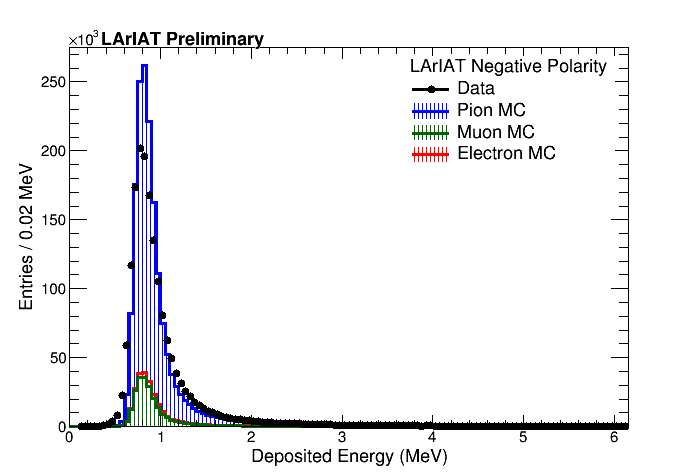
\includegraphics[width=0.48\textwidth]{Studies/Figures/DepEnergy_Stacked_v1.png}
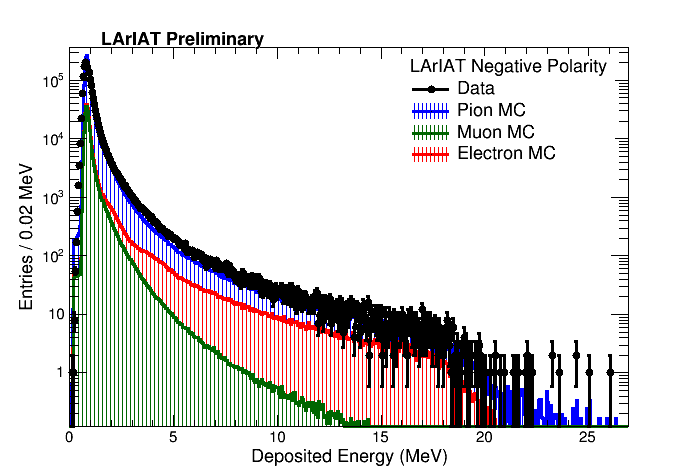
\includegraphics[width=0.48\textwidth]{Studies/Figures/DepEnergy_Stacked_v3.png}
\caption[]{ Energy Deposited with all the MC and 60A data.  } \label{fig:EnergyDepositedStacked}
\end{figure}

The energy at the interacting point is given by
\begin{equation}
KE_{Interaction} = \sqrt{P_{WCtrk}^2 + m_{\pi}^2} - E_{Loss} - (\Sigma dE/dX_{i} \times Pitch)
\end{equation}

and has the exact same uncertainty as the incident kinetic energy plot. Thus these estimates can be applied to getting the uncertainty on the energy of the reconstructed cross-section.

